\chapter{Resultados}
  En esta investigación, se expondrán dos redes neuronales, diferenciadas por el hecho de que en una de ellas se duplicaron los pesos. Este ajuste se llevó a cabo con el propósito de evaluar en qué medida el aprendizaje incremental impacta en el rendimiento de una red neuronal.

  Para la construcción de estas redes, se emplearon datos del conjunto de datos Optical Digit, el cual proporciona la información necesaria para el entrenamiento de la red neuronal. Todo el proceso se llevó a cabo en el entorno virtual de Google Colab utilizando la biblioteca Tensorflow.

  A continuación, se presentarán los resultados obtenidos de la red neuronal que no experimentó la duplicación de pesos. Esta red puede ser descrita como simple, al menos en comparación con su contraparte modificada.

  \begin{figure}[H]
    \centering
    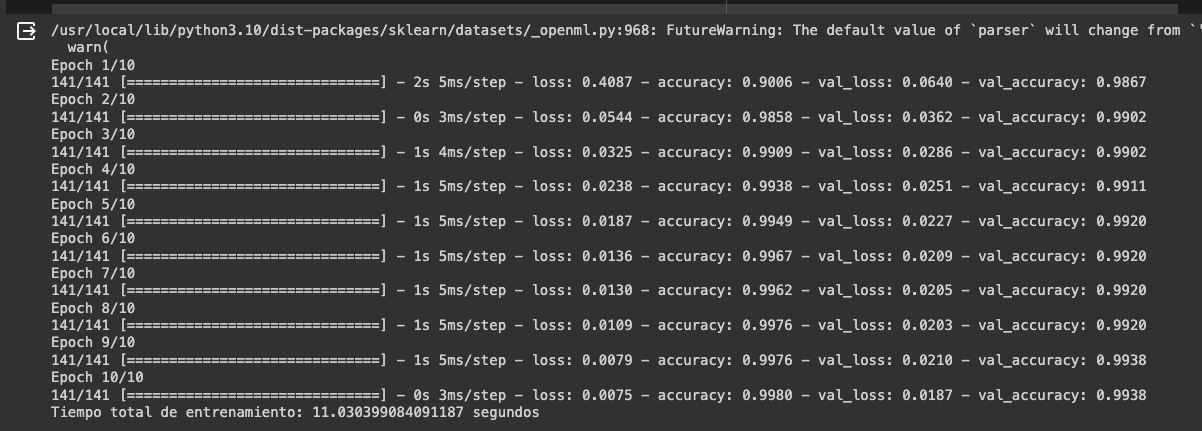
\includegraphics[width=\columnwidth]{firstResullt.png}
    \caption{Primeros Resultados}
    \label{fig: first result and time}
  \end{figure}

  Tal como se puede apreciar en la imagen \ref{fig: first result and time}  previa, se evidencia que el tiempo de ejecución registrado fue de 11 segundos. Esta métrica temporal proporciona una indicación clara del rendimiento y eficiencia del proceso, siendo un factor relevante para evaluar la eficacia de la tarea realizada. La breve duración del tiempo de ejecución sugiere una ejecución rápida y eficiente de la operación en cuestión, lo cual puede ser un aspecto positivo en términos de eficacia y velocidad de respuesta del sistema o del algoritmo implementado.

  A continuación, se procederá a examinar la precisión por época, la pérdida por época y cómo evoluciona su precisión a lo largo de las iteraciones. Este análisis proporcionará una visión detallada de la dinámica del modelo a medida que avanza en el proceso de entrenamiento. Observar la relación entre estas métricas a lo largo de las iteraciones permitirá entender mejor la capacidad de aprendizaje y la convergencia del modelo, ofreciendo insights cruciales sobre su desempeño en el conjunto de datos. Este enfoque detallado en las métricas temporales y su evolución es esencial para una evaluación integral del rendimiento del modelo a lo largo del tiempo.

  \begin{figure}[H]
    \centering
    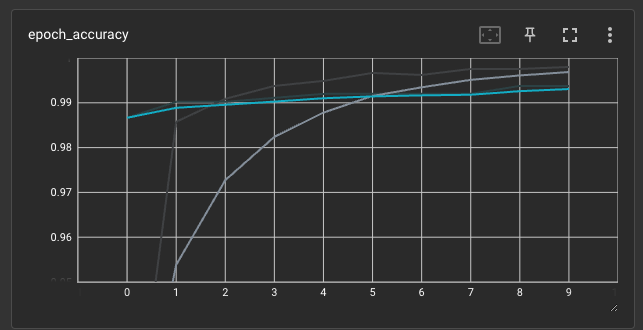
\includegraphics[width=\columnwidth]{epochAccuracy.png}
    \caption{Precisión por época}
    \label{fig: epochAccuracy}
  \end{figure}

  \begin{figure}[H]
    \centering
    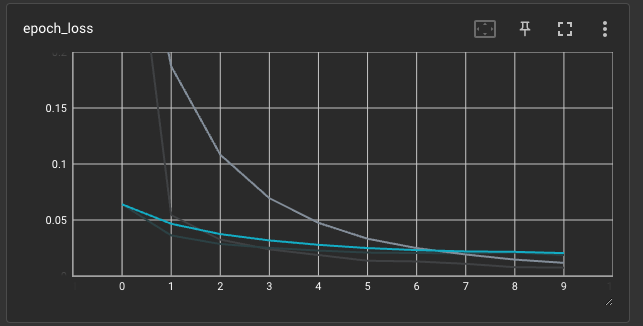
\includegraphics[width=\columnwidth]{epochLoss.png}
    \caption{Perdida por época}
    \label{fig: epochLoss}
  \end{figure}

  \begin{figure}[H]
    \centering
    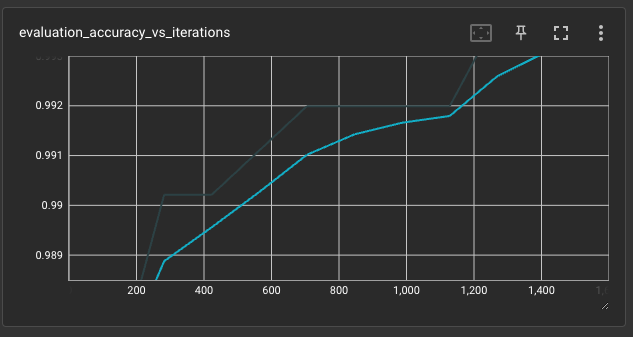
\includegraphics[width=\columnwidth]{evaluationAccuracyvsIterations.png}
    \caption{Evaluación en la precisión}
    \label{fig: evaluationAccuracyvsIterations}
  \end{figure}

  La observación detallada de la evaluación de esta red neuronal revela un progreso positivo a lo largo del tiempo. Se aprecia una tendencia favorable en la mejora de las métricas, indicando un rendimiento en constante optimización. Es destacable notar que la pérdida de información exhibe una disminución constante, lo cual sugiere una eficaz capacidad de aprendizaje de la red. Este patrón descendente en la pérdida señala que la red está refinando su capacidad para representar y generalizar patrones, lo cual es crucial para un rendimiento robusto en diversas situaciones. En resumen, los indicios visibles apuntan a una evolución positiva y a una mejora progresiva en la capacidad predictiva de la red neuronal.

  En el próximo paso de la investigación, se llevará a cabo el mismo procedimiento, pero con la única variación de aumentar los pesos en la red neuronal. Esta modificación busca explorar y comparar las diferencias resultantes entre ambas configuraciones. Al introducir este ajuste específico, se espera identificar de manera clara y específica cómo el incremento de los pesos afecta las métricas de rendimiento, como la precisión y la pérdida. Este enfoque comparativo permitirá discernir el impacto singular de esta modificación en el comportamiento y la eficacia del modelo, proporcionando información valiosa sobre la influencia directa de los pesos en la capacidad de aprendizaje y generalización de la red neuronal.

  \begin{figure}[H]
    \centering
    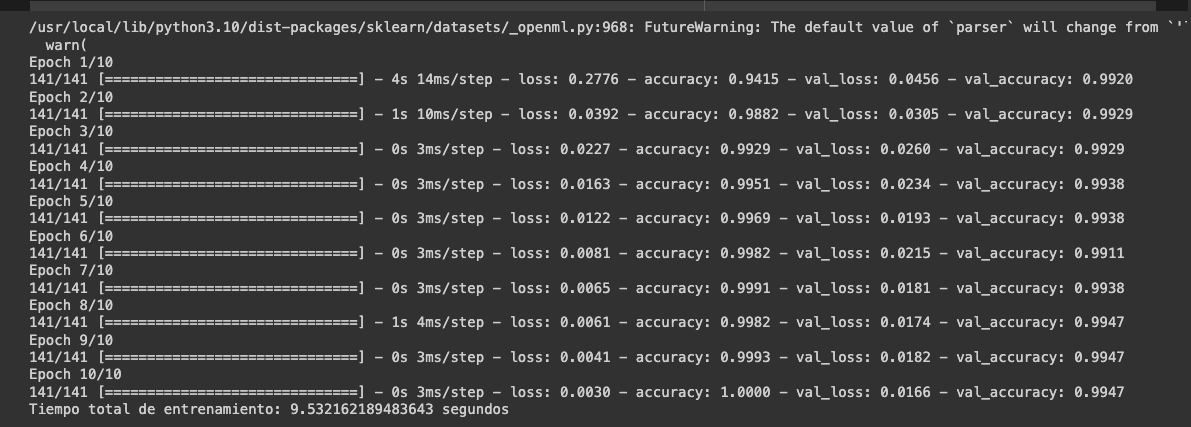
\includegraphics[width=\columnwidth]{secondResult.png}
    \caption{Segundos Resultados}
    \label{fig: second result and time}
  \end{figure}

  En el análisis de los resultados, se destaca una diferencia significativa, siendo notable que el tiempo de ejecución se reduce a dos segundos. Este cambio representa una ventaja considerable en términos de eficiencia temporal. La disminución en el tiempo de ejecución sugiere una mejora en la velocidad de procesamiento al aumentar los pesos en la red neuronal. Esta eficiencia temporal puede ser una consideración crucial, especialmente en entornos donde la rapidez en la obtención de resultados es esencial. La reducción del tiempo de ejecución a dos segundos podría traducirse en un beneficio operativo notable, optimizando el rendimiento general del modelo y acelerando el proceso de toma de decisiones.  

  Ahora examinaremos detenidamente la presión, la pérdida de la época y también observaremos cómo evoluciona la precisión en relación con este resultado innovador. Nos enfocaremos en analizar minuciosamente cada aspecto, permitiéndonos comprender de manera más exhaustiva la influencia de estos elementos en el nuevo resultado que estamos obteniendo.

  \begin{figure}[H]
    \centering
    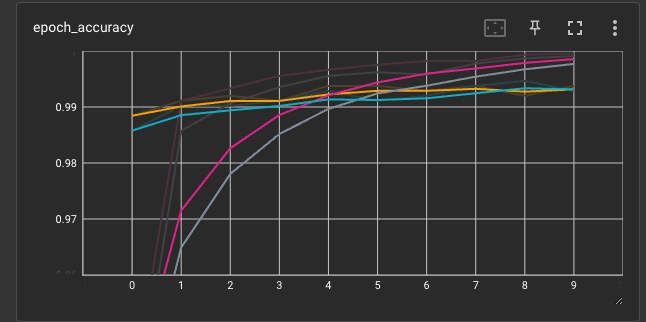
\includegraphics[width=\columnwidth]{epochAccuracySecondNN.png}
    \caption{Precisión de época con pesos duplicados}
    \label{fig: epochAccuracySecondNN}
  \end{figure}

  \begin{figure}[H]
    \centering
    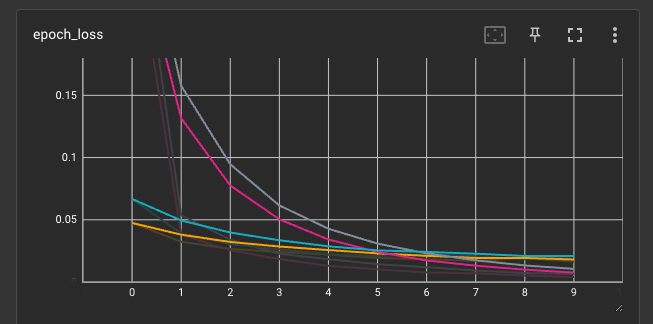
\includegraphics[width=\columnwidth]{epochLossSecondNN.png}
    \caption{Perdida de época}
    \label{fig: epochLossSecondNN}
  \end{figure}

  \begin{figure}[H]
    \centering
    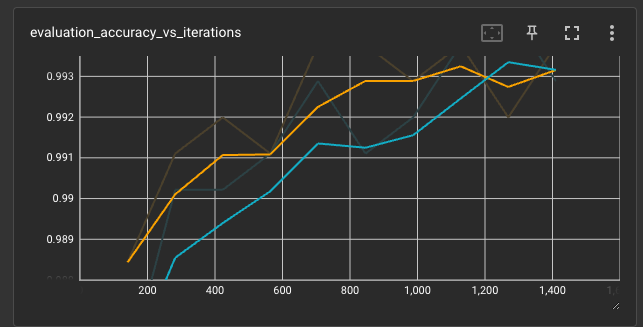
\includegraphics[width=\columnwidth]{evalutionAccuracyvsIterationSeoondNN.png}
    \caption{Evaluación en la precisión}
    \label{fig: evalutionAccuracyvsIterationSeoondNN}
  \end{figure}

  Al analizar las representaciones gráficas proporcionadas a través de TensorBoard, se evidencian notables disparidades, siendo una de las más destacadas la presencia de un mayor número de capas ocultas. Estas capas adicionales se visualizan mediante líneas de colores distintos, y al evaluarlas, se observa una marcada diferencia. Se destaca que varias de estas capas adicionales exhiben una mayor precisión durante el proceso de entrenamiento.

  En resumen, al duplicar los pesos de una red neuronal, se percibe una mejora sustancial en su rendimiento. Esta estrategia se revela como eficaz y eficiente, aunque conlleva un tiempo de entrenamiento ligeramente más prolongado en comparación con una red convencional. Al realizar la evaluación, se constata que la precisión de la red con pesos duplicados supera significativamente a la de una red convencional.